\subsection{M.PC.1 - Percentuale di metriche soddisfatte}
\begin{figure}[H]
    \centering
    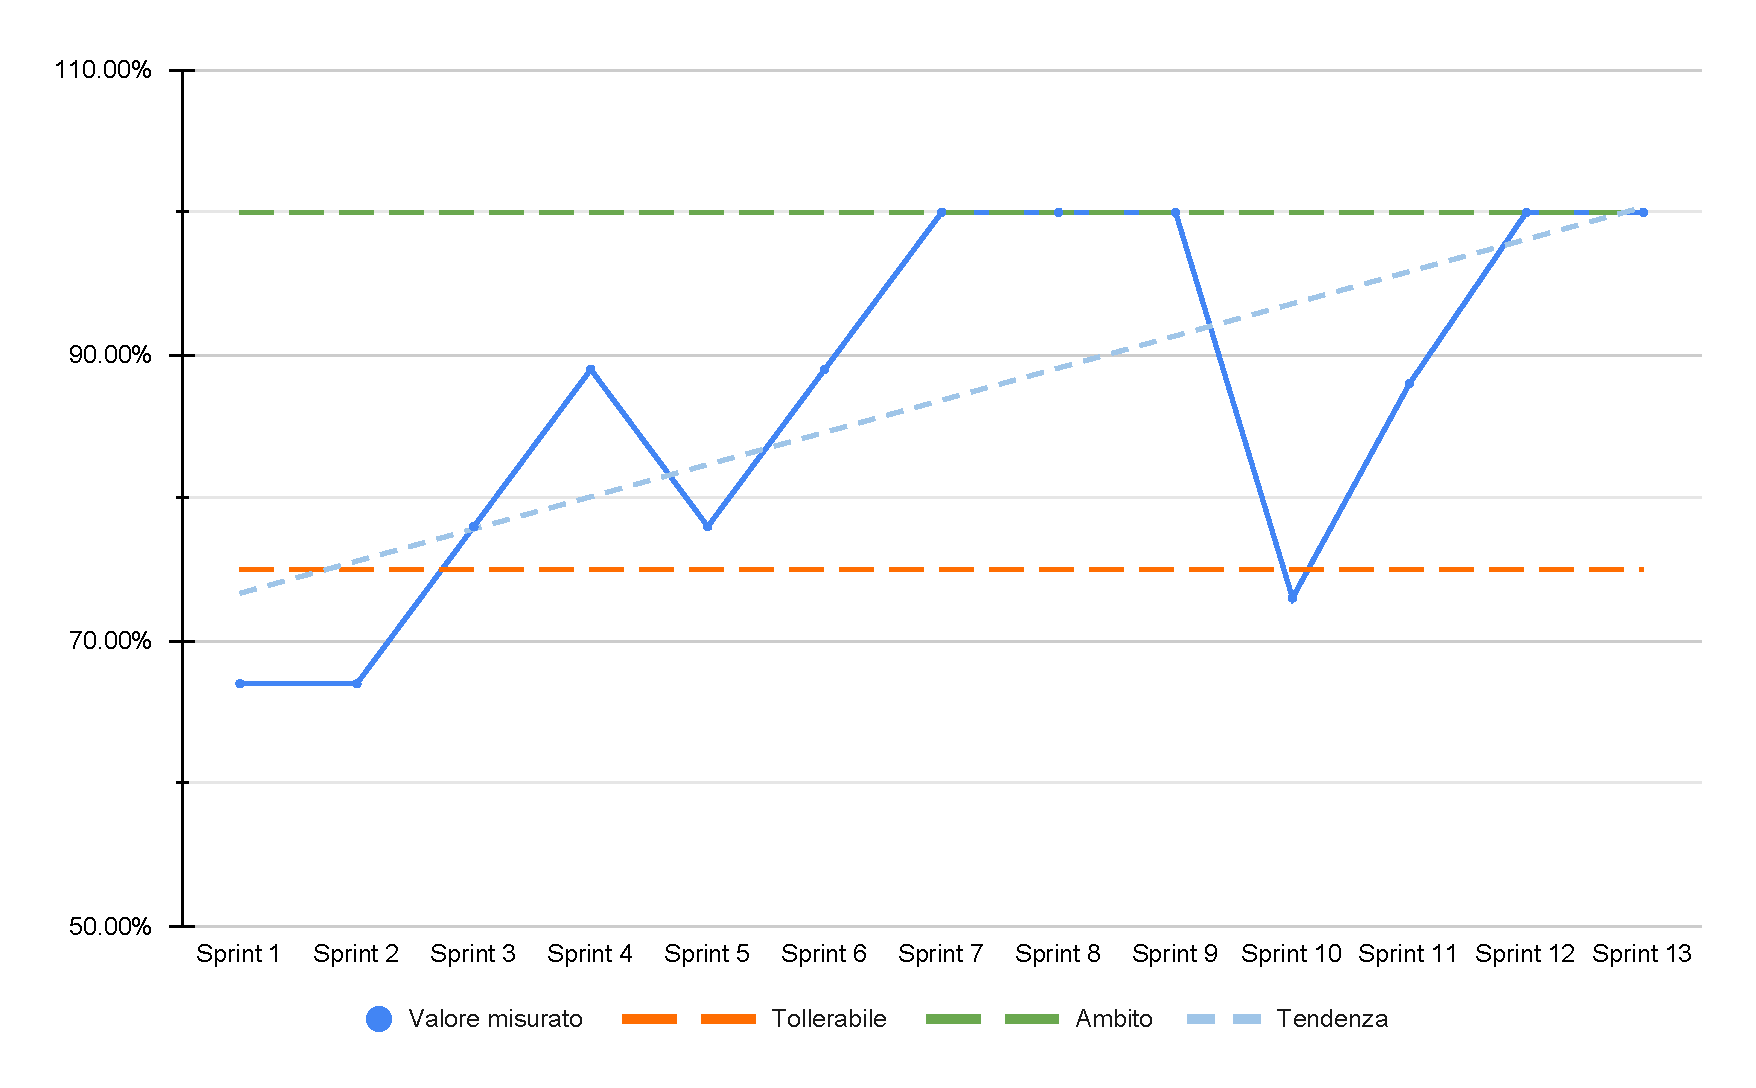
\includegraphics[width=\textwidth]{assets/metriche_soddisfatte.pdf}
    \caption{M.PC.1 - Percentuale di metriche soddisfatte}
\end{figure}

\par Il grafico sottolinea come negli \glossario{sprint} iniziali il team non abbia raggiunto la soglia di tollerabilità stabilita. Il mancato raggiungimento degli obiettivi era dovuto all'inesperienza del gruppo e alla difficoltà di adattamento ai processi di lavoro e alle pratiche dell'ingegneria del software. Tuttavia, nel corso degli \glossario{sprint} successivi, il gruppo ha notato dei progressi, specie nell'ottemperanza alle metriche di variazione del piano e del budget. Questo è dovuto all'introduzione di feedback migliorativi, alla maggiore competenza e collaborazione all'interno del team, e all'applicazione più puntuale del ciclo di PDCA. Inoltre, il gruppo ha aggiornato e approfondito il \WoW\ nelle \NdP, incrementando la qualità dei processi. Il grafico illustra un miglioramento costante nel tempo, fino a raggiungere il valore ambito nel settimo sprint. Già dal terzo sprint, però, il valore misurato era superiore alla soglia considerata tollerabile. 

\par Con l'introduzione del monitoraggio delle metriche di prodotto, il team è riuscito a mantenere un livello di qualità costante. L'unica eccezione si è verificata durante il decimo \glossario{sprint}, in cui la percentuale di metriche soddisfatte è scesa al di sotto della soglia accettabile. Questo calo è dovuto all'inesperienza del gruppo nelle fasi di progettazione e testing, fondamentali per il raggiungimento degli standard previsti. A partire dallo sprint 12, tuttavia, la percentuale di metriche soddisfatte è tornata al 100\%.
